\documentclass{standalone}
\usepackage{graphicx}	
\usepackage{amssymb, amsmath}
\usepackage{color}

\usepackage{tikz}
\usetikzlibrary{intersections, backgrounds}

\definecolor{light}{RGB}{220, 188, 188}
\definecolor{mid}{RGB}{185, 124, 124}
\definecolor{dark}{RGB}{143, 39, 39}
\definecolor{highlight}{RGB}{180, 31, 180}
\definecolor{gray10}{gray}{0.1}
\definecolor{gray20}{gray}{0.2}
\definecolor{gray30}{gray}{0.3}
\definecolor{gray40}{gray}{0.4}
\definecolor{gray60}{gray}{0.6}
\definecolor{gray70}{gray}{0.7}
\definecolor{gray80}{gray}{0.8}
\definecolor{gray90}{gray}{0.9}
\definecolor{gray95}{gray}{0.95}

\newcommand*{\offset}{0.025}

\begin{document}

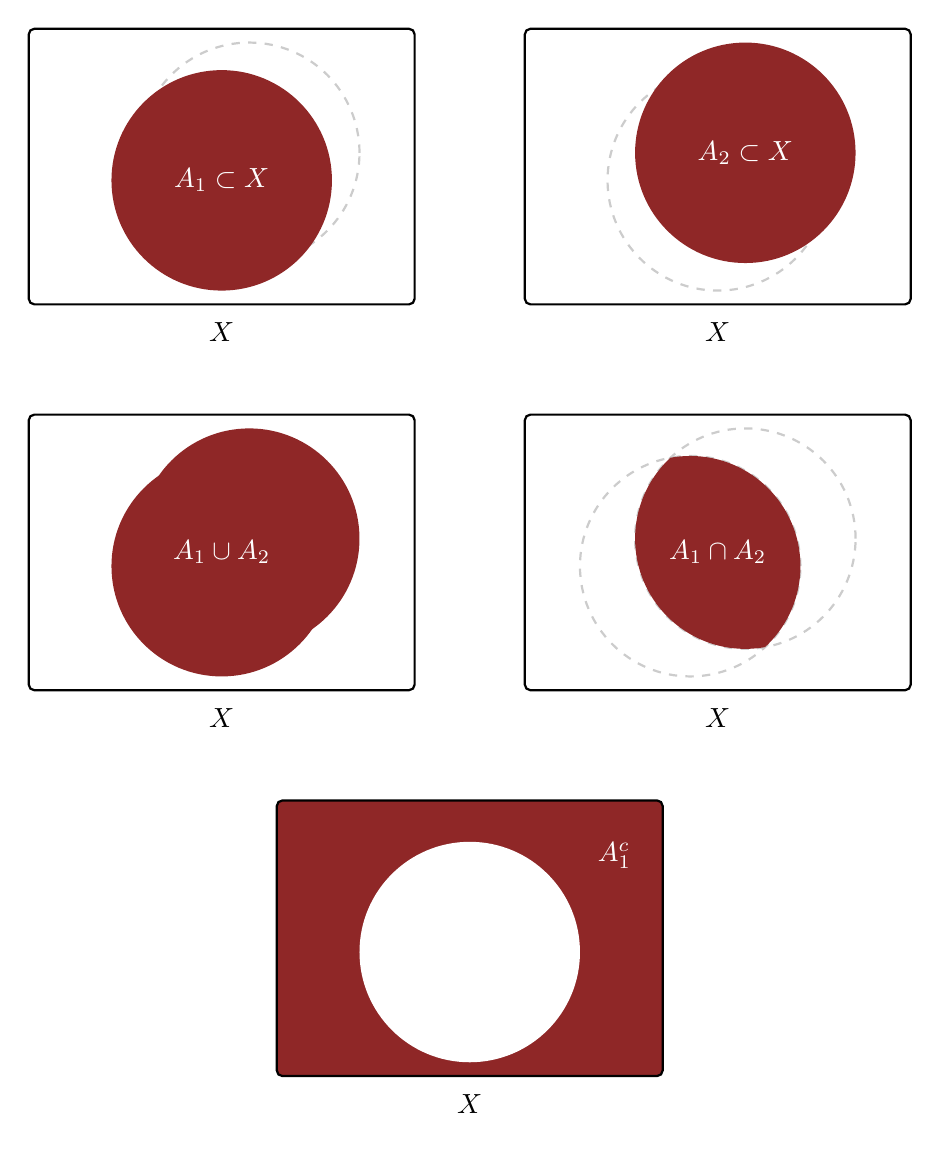
\begin{tikzpicture}[scale=0.35, thick]
  % Set A
  \draw [rounded corners=2pt, color=black] (-2, 0) rectangle +(-14, 10);
  \node at (-9, -1) { $X$ };

  \draw [color=gray80, dashed] (-8, 5.5) circle (4); 
  \fill [color=dark, text=white] (-9, 4.5) circle (4) node {$A_{1} \subset X$}; 
  
  % Set B
  \draw [rounded corners=2pt, color=black] (2, 0) rectangle +(14, 10);
  \node at (9, -1) { $X$ };
  
  \draw [color=gray80, dashed] (9, 4.5) circle (4); 
  \fill [color=dark, text=white] (10, 5.5) circle (4) node {$A_{2} \subset X$}; 

  % Set Union
  \draw [rounded corners=2pt, color=black] (-2, -14) rectangle +(-14, 10);
  \node at (-9, -15) { $X$ };

  \fill [color=dark] (-9, -9.5) circle (4); 
  \fill [color=dark] (-8, -8.5) circle (4); 
  \node [text=white] at (-9, -9) {$A_{1} \cup A_{2}$};
  
  % Set Intersection
  \draw [rounded corners=2pt, color=black] (2, -14) rectangle +(14, 10);
  \node at (9, -15) { $X$ };
  
  \draw [color=gray80, dashed] (8, -9.5) circle (4); 
  \draw [color=gray80, dashed] (10, -8.5) circle (4);   
  
  \begin{scope}
  	\clip (8, -9.5) circle (4);
	\fill [color=dark] (10, -8.5) circle (4);
  \end{scope}
  \node [text=white] at (9, -9) {$A_{1} \cap A_{2}$};
  
  % Set Complement
  \fill [rounded corners=2pt, color=dark] (-7, -28) rectangle +(14, 10);
    
  \draw [rounded corners=2pt, color=black] (-7, -28) rectangle +(14, 10);
  \node at (0, -29) { $X$ };
  
  \fill [color=white] (0, -23.5) circle (4);
  \node[color=white] at (5.25, -20) {$A_{1}^{c}$};
  
\end{tikzpicture}

\end{document}  